\documentclass[12pt,a4paper]{article}
\usepackage[utf8]{inputenc}
\usepackage[magyar]{babel}
\usepackage[T1]{fontenc}
\usepackage{graphicx}
\usepackage[left=2cm,right=2cm,top=2cm,bottom=2cm]{geometry}
\begin{document}

\centering\Large\textbf{Témalabor: rókavevő + teszt adó - HVT 2018}

\begin{figure}[!h]
\centering
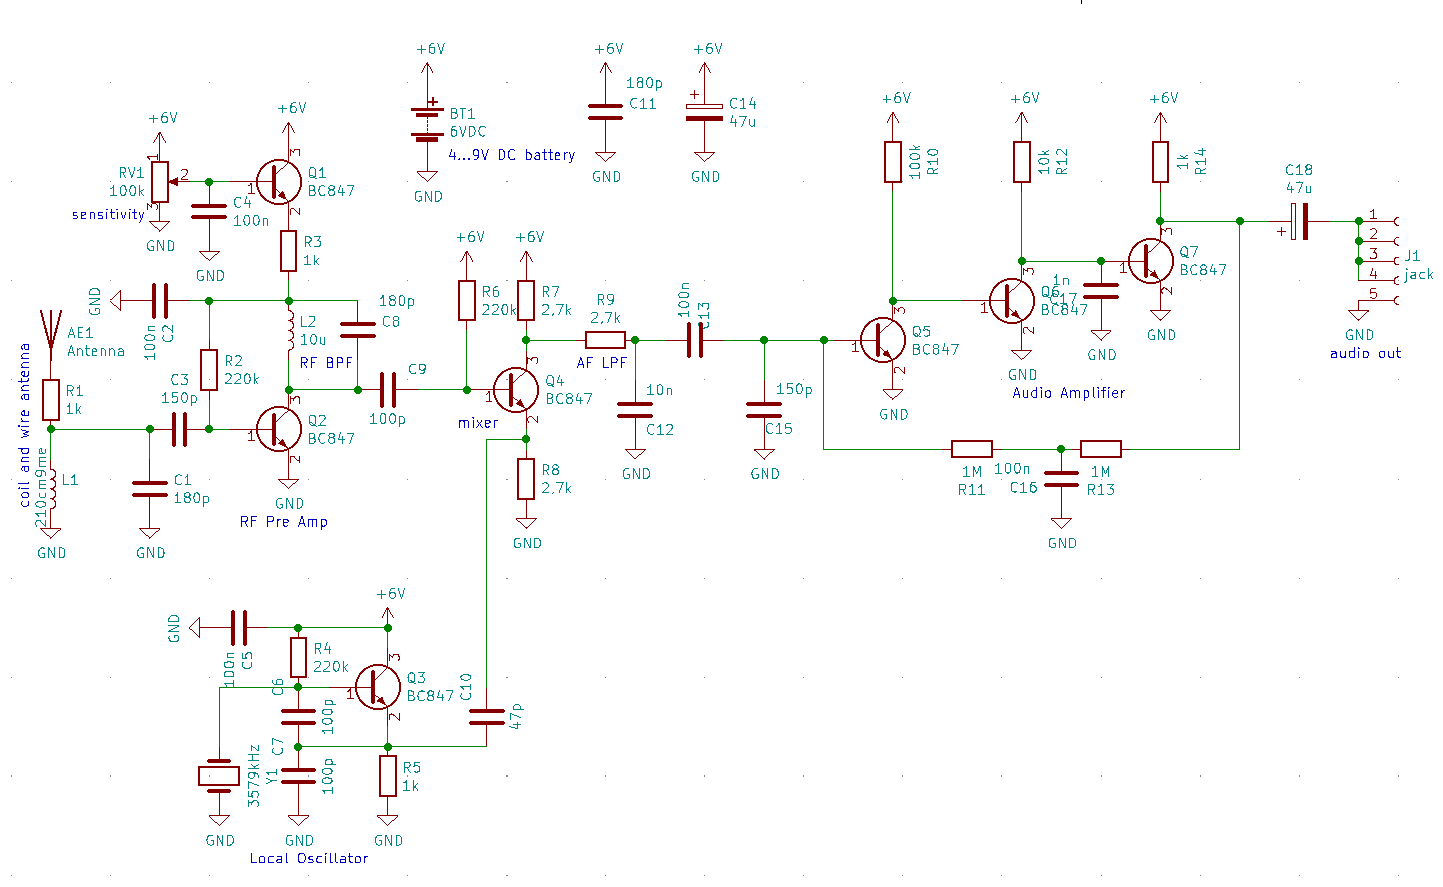
\includegraphics[width=1\textwidth]{../pic/sch.png}
\caption{A rókavevő kapcsolási rajza}
\end{figure}

\begin{figure}[!h]
\centering
\includegraphics[width=.6\textwidth]{../pic/ult2x.png}
\includegraphics[width=.3\textwidth]{../pic/alk.png}
\caption{Alkatrész ültetési rajz és alkatrész lista}
\end{figure}

\end{document}